

\section{Background and Motivation}

Every option trade has a buyer and seller side. For a plethora of problems in option research, it’s also crucial to determine the party that initiated the transaction. Applications include the study of option demand \autocite[][]{garleanuDemandBasedOptionPricing2009}, of informational content in option trading \autocites[][]{huDoesOptionTrading2014}[][]{panInformationOptionVolume2006}[][]{caoInformationalContentOption2005}, of order flow \autocite[][]{muravyevOrderFlowExpected2016}, or of trading costs \autocite[][]{muravyevOptionsTradingCosts2020}. 

Despite the clear importance for empirical research, the true initiator of the trade is frequently absent in datasets and is inferred using trade classification rules \autocite[][]{easleyOptionVolumeStock1998}. In consequence, the correctness of empirical studies hinges on the algorithm's ability to accurately identify the trade initiator.

Popular heuristic to sign trades are the tick test \autocite[][]{hasbrouckTradesQuotesInventories1988}, quote rule \autocite[][]{harrisDayEndTransactionPrice1989}, and hybrids thereof such as the \gls{LR} algorithm \autocite[][]{leeInferringTradeDirection1991}. These rules have initially been proposed and tested in the stock market. For option markets, the works of \textcites[][]{savickasInferringDirectionOption2003}[][]{grauerOptionTradeClassification2022} raise concerns about the transferability of trade signing rules due to deteriorating classification accuracies and systematic misclassifications. The latter is crucial, as non-random misclassifications bias the dependent research \autocites[][]{odders-whiteOccurrenceConsequencesInaccurate2000}[][]{theissenTestAccuracyLee2001}.

A second, growing body of research \autocites{blazejewskiLocalNonParametricModel2005}{rosenthalModelingTradeDirection2012}{ronenMachineLearningTrade2022} advances trade classification performance through \gls{ML}. The scope of current works is yet bound to the stock market and the superficial setting, where supervised models are trained on fully-labeled trades. Then again, labeled trades are difficult to obtain, whereas unlabeled trades are abundant.

The goal of our empirical study is to investigate if a \gls{ML}-based classifier can improve upon the accuracy of state-of-the-art approaches in option trade classification.

\section{Contributions}

Our contributions are three-fold: 
\begin{enumerate}[label=(\roman*),noitemsep]
\item By employing \glspl{GBRT} and transformers we establish a new state-of-the-art in option trade classification. We outperform existing approaches by \SI{3.73}{\percent}~-~\SI{6.51}{\percent} in accuracy on a large sample of \gls{ISE} trades. Relative to the ubiquitous \gls{LR} algorithm, improvements are up to \SI{17.02}{\percent}. 
The model's efficacy is demonstrated for alternative trading venues, in sub-samples, and in an application study.
\item Our work is the first to consider trade classification also in the semi-supervised scenario, where trades are only partially labeled. Our best models classify \SI{74.55}{\percent} (+ 6.94) of all trades correctly.
\item Through a feature importance analysis based on Shapley values, we can consistently attribute performance gains of rule-based and \gls{ML}-based classifiers to feature groups. We discover that both paradigms share common features, but \gls{ML}-based approaches more effectively exploit the data.
\end{enumerate}

\section{Data}

We perform the empirical analysis on two large-scale datasets of option trades recorded at the \gls{ISE} and \gls{CBOE}. Our sample construction follows \textcite[][]{grauerOptionTradeClassification2022}, which fosters comparability between both works. 

Training and validation are performed exclusively on \gls{ISE} trades. After a time-based train-validation-test split (\SI{60}{\percent}; \SI{20}{\percent}; \SI{20}{\percent}), required by the \gls{ML} estimators, we are left with a test set spanning from Nov. 2015 -- May 2017 at the \gls{ISE}. \gls{CBOE} trades between Nov. 2015 -- Oct. 2017 are used as a second test set. Each test set contains between 9.8 Mio. --  12.8 Mio. labeled option trades. An additional unlabeled, training set of \gls{ISE} trades executed between Oct. 2012 -- Oct. 2013 is reserved for learning in the semi-supervised setting.

To establish a common ground with rule-based classification, we distinguish three feature sets with increasing data requirements and employ minimal feature engineering. The first set is based on the data requirements of tick/quote-based algorithms, the second of hybrid algorithms with additional dependencies on trade size data, such as the \gls{GSU} method \autocite{grauerOptionTradeClassification2022}, and the third feature set includes option characteristics, like the option's $\Delta$ or the underlying. 

\section{Methodology}

We model trade classification using \glspl{GBRT} \autocites[][]{friedmanGreedyFunctionApproximation2001}, a wide tree-based ensemble, and the FT-Transformer \autocite{gorishniyRevisitingDeepLearning2021}, a Transformer-based neural network architecture. We select these approaches for their state-of-the-art performance in tabular modeling \autocites[][]{gorishniyRevisitingDeepLearning2021}[][]{grinsztajnWhyTreebasedModels2022} and their extendability to learn on partially-labeled trades. Additionally, Transformers offer \textit{some} model interpretability through the Attention mechanism. An advantage we exploit later to derive insights into the classification process of Transformers.

As stated earlier, our goal is to extend \gls{ML} classifiers for the semi-supervised setting to make use of the abundant, unlabeled trade data. We couple gradient-boosting with self-training \autocite{yarowskyUnsupervisedWordSense1995}, whereby confident predictions of unlabeled trades are iteratively added into the training set as pseudo-labels. A new classifier is then retrained on labeled and pseudo-labeled trades. Likewise, the Transformer is pre-trained on unlabeled trades with the replaced token detection objective \autocite{clarkElectraPretrainingText2020} and later finetuned on labeled training instances. Conceptually, the network is tasked to detect randomly replaced tokens or features of transactions. Both techniques are aimed at improving generalization performance.

Classical trade classification rules are implemented as a rule-based classifier allowing us to construct arbitrary candidates for benchmarking and support richer evaluation of feature importances.\footnote{Our implementation is publically available under \url{https://pypi.org/project/tclf/}.}

To facilitate a fair comparison, we run an exhaustive Bayesian search, to find a suitable hyperparameter configuration for each of our models. Classical
rule have no hyperparameters per se. Akin to tuning the \gls{ML} classifiers on the validation set, we select candidate rules the classical benchmarks based on their validation performance. This is most rigorous while preventing overfitting the test set.\footnote{All of our source code and experiments are publically available under \url{https://github.com/KarelZe/thesis/}.}

\section{Results}

\begin{table*}
    \centering
    \caption[Accuracies of Supervised Classifiers]{Accuracy of supervised \glspl{GBRT} and Transformers for different feature combinations on the \gls{ISE} and \gls{CBOE} datasets. The improvement is estimated as the absolute change in accuracy between the classifier and the benchmark. For the feature set classic \gls{GSU} (small) is the benchmark and otherwise \gls{GSU} (large). Models are trained on the \gls{ISE} training set. The best classifier per dataset is in \textbf{bold}.}
    \label{tab:results-supervised-ise-cboe}
    \begin{tabular}{@{}llSSSSSS@{}}
        \toprule
                   &             & \multicolumn{2}{c}{\glsentryshort{FS} Classic} & \multicolumn{2}{c}{\glsentryshort{FS} Size} & \multicolumn{2}{c}{\glsentryshort{FS} Option}                                                                 \\ \cmidrule(lr){3-4}\cmidrule(lr){5-6} \cmidrule(lr){7-8}
        Dataset    & Classifier  & {Acc. in \%}                                     & {+/-}                                                 & {Acc. in \%}                                  & {+/-}              & {Acc. in \%}        & {+/-}              \\ \midrule
        \gls{ISE}  & \gls{GBRT}  & 63.668637                                        & 3.620000                                              & 72.343640                                     & 4.730000           & \bfseries 74.120496 & \bfseries 6.510000 \\
                   & Transformer & \bfseries 63.783020                              & \bfseries 3.730000                                    & \bfseries 72.581107                           & \bfseries 4.970000 & 73.921795           & 6.310000           \\ \addlinespace
        \gls{CBOE} & \gls{GBRT}  & 66.002029                                        & 5.260000                                              & 71.951794                                     & 5.430000           & \bfseries 74.375033 & \bfseries 7.860000 \\
                   & Transformer & \bfseries 66.182348                              & \bfseries 5.440000                                    & \bfseries 72.153338                           & \bfseries 5.640000 & 74.278318           & 7.760000           \\ \bottomrule
    \end{tabular}
\end{table*}


\begin{table*}
    \centering
    \caption[Accuracies of Semi-Supervised Classifiers]{Accuracy of semi-supervised \glspl{GBRT} and Transformers for different feature combinations on the \gls{ISE} and \gls{CBOE} datasets. The improvement is estimated as the absolute change in accuracy between the classifier and the benchmark. For the feature set classic \gls{GSU} (small) is the benchmark and otherwise \gls{GSU} (large). Models are trained on the \gls{ISE} training set. The best classifier per dataset is in \textbf{bold}.}
    \label{tab:results-semi-supervised-ise-cboe}
    \begin{tabular}{@{}llSSSSSS@{}}
        \toprule
                   &             & \multicolumn{2}{c}{\glsentryshort{FS} Classic} & \multicolumn{2}{c}{\glsentryshort{FS} Size} & \multicolumn{2}{c}{\glsentryshort{FS} Option}                                                                 \\ \cmidrule(lr){3-4}\cmidrule(lr){5-6} \cmidrule(lr){7-8}
        Dataset    & Classifier  & {Acc. in \%}                                     & {+/-}                                                 & {Acc. in \%}                                  & {+/-}              & {Acc. in \%}        & {+/-}              \\ \midrule
        \gls{ISE}  & \gls{GBRT}  & 63.397514                                        & 3.350000                                              & 72.156489                                     & 4.550000           & 73.536644           & 5.930000           \\
                   & Transformer & \bfseries 64.655751                              & \bfseries 4.600000                                    & \bfseries 72.859054                           & \bfseries 5.250000 & \bfseries 74.551410 & \bfseries 6.940000 \\ \addlinespace
        \gls{CBOE} & \gls{GBRT}  & \bfseries 66.189454                              & \bfseries 5.440000                                    & \bfseries 71.922680                           & \bfseries 5.410000 & 73.953322           & 7.440000           \\
                   & Transformer & 65.668441                                        & 4.920000                                              & 71.783984                                     & 5.270000           & \bfseries 74.095833 & \bfseries 7.580000 \\ \bottomrule
    \end{tabular}
\end{table*}

For an evaluation of feature importances, that suffices for a cross-model comparison, we use \gls{SAGE} \autocite{covertUnderstandingGlobalFeature2020}. It is a global feature importance measure based on Shapley values and capable of handling complex feature interaction, such as highly correlated quotes and prices. We estimate \gls{SAGE} values in terms of improvement in zero-one loss per feature set, complementing our accuracy-based evaluation.

\begin{figure*}[h]
    \centering
    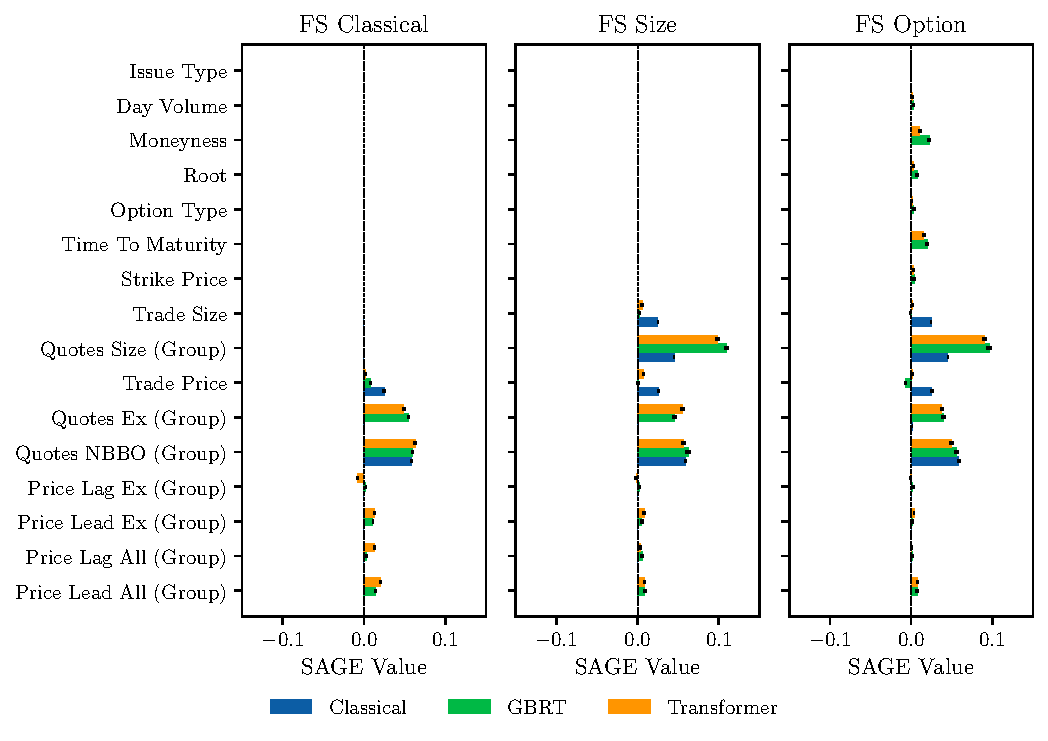
\includegraphics[width=1\textwidth]{sage-importances.pdf}
    \caption[\glsentryshort{SAGE} Feature Importances]{\gls{SAGE} feature importances of rule-based and \gls{ML}-based classifiers. Importances estimated on \gls{ISE} test set with zero-one loss. Bigger feature importances are better. For feature set classical the \gls{GSU} method (small) is used and otherwhise the \gls{GSU} method (large).}
    \label{fig:sage-importances}
\end{figure*}

As visible from \cref{fig:sage-importances} we find, that all models attain the largest improvement in loss from quoted prices and if provided from the quoted sizes. The contribution of the \gls{NBBO} to performance is roughly equal for all models, suggesting that even simple heuristics effectively exploit the data. For \gls{ML}-based predictors, quotes at the exchange level hold equal importance in classification. This contrasts with \gls{GSU} methods, which rely less on exchange-level quotes.  The performance improvements from the trade size and quoted size, are slightly lower for rule-based methods compared to \gls{ML}-based methods. Transformers and \glspl{GBRT} slightly benefit from the addition of option features, i.e., moneyness and time to maturity. 

Regardless of the method used, changes in trade price, central to the tick test, are irrelevant for classification and can even harm performance. This result alligns with earlier studies of \textcites{savickasInferringDirectionOption2003}{grauerOptionTradeClassification2022}.

In summary,\dots

An interesting venue for future research is to \dots
% Similarly, additional features such as option type, issue type, the trading volume of the option series, and the underlying are also irrelevant. 
% Overall, we observe a large agreement between the importance of features in classical trade classification rules and machine learning-based predictors.


% Following good measures, we perform robustness tests across different sub-samples such as option type, type of underlying, and time among others. 
% % We demonstrate its efficacy by evaluating on the problem of click fraud detection on ads to obtain a 9% relative improvement on robot detection metrics over a supervised learning baseline and 4% over a contrastive learning experiment.

% But unlike these

% spurting its growth


% \section{Relevancy}
